% Gemini theme
% https://github.com/anishathalye/gemini

\documentclass[final]{beamer}

% ====================
% Packages
% ====================

\usepackage[T1]{fontenc}
\usepackage{lmodern}
\usepackage[size=a0,scale=1.0, orientation=portrait]{beamerposter}
\usetheme{gemini}
\usecolortheme{gemini}
%\usecolortheme{custom}
\usepackage{graphicx}
\usepackage{booktabs}
\usepackage{tikz}
\usepackage{pgfplots}
\usepackage{amsmath} % assumes amsmath package installed
\usepackage{amssymb}  % assumes amsmath package installed
\usepackage{multirow}
\usepackage{tabularx}

\graphicspath{{../slides/}}

% ====================
% Lengths
% ====================

% If you have N columns, choose \sepwidth and \colwidth such that
% (N+1)*\sepwidth + N*\colwidth = \paperwidth
\newlength{\sepwidth}
\newlength{\colwidth}
\setlength{\sepwidth}{0.025\paperwidth}
\setlength{\colwidth}{0.3\paperwidth}

\newcommand{\separatorcolumn}{\begin{column}{\sepwidth}\end{column}}
\newcommand{\norm}[1]{\left\lVert#1\right\rVert}

% ====================
% Title
% ====================

\title{Learning Scene Geometry for Visual Localization in Challenging Conditions}

\author{Nathan Piasco\inst{1, 2} \and Désiré Sidibé \inst{1} \and Valérie Gouet-Brunet \inst{2} and Cédric Demonceaux  \inst{1}}

\institute[shortinst]{\inst{1} ImViA-VIBOT, ERL CNRS 6000, Université Bourgogne Franche-Comtée \samelineand \inst{2} LaSTIG MATIS, IGN, ENSG, Université Paris-Est, F-94160 Saint-Mandé, France}

% ====================
% Body
% ====================

\begin{document}

\begin{frame}[t]
\begin{columns}[t]
\separatorcolumn

\begin{column}{\colwidth}
  \begin{alertblock}{Abstract}

	  We propose a new approach for outdoor large scale image based localization that can deal with challenging scenarios like cross-season, cross-weather, day/night and long-term localization. The key component of our method is a new learned global image descriptor, that can effectively benefit from scene geometry information during training. At test time, our system is capable of inferring the depth map related to the query image and use it to increase localization accuracy.

  \end{alertblock}
  
  \vspace{2cm}

  \begin{block}{Problem statement}

	We want to find the position of an image query according to a known reference.
	
    \begin{figure}
      \centering
      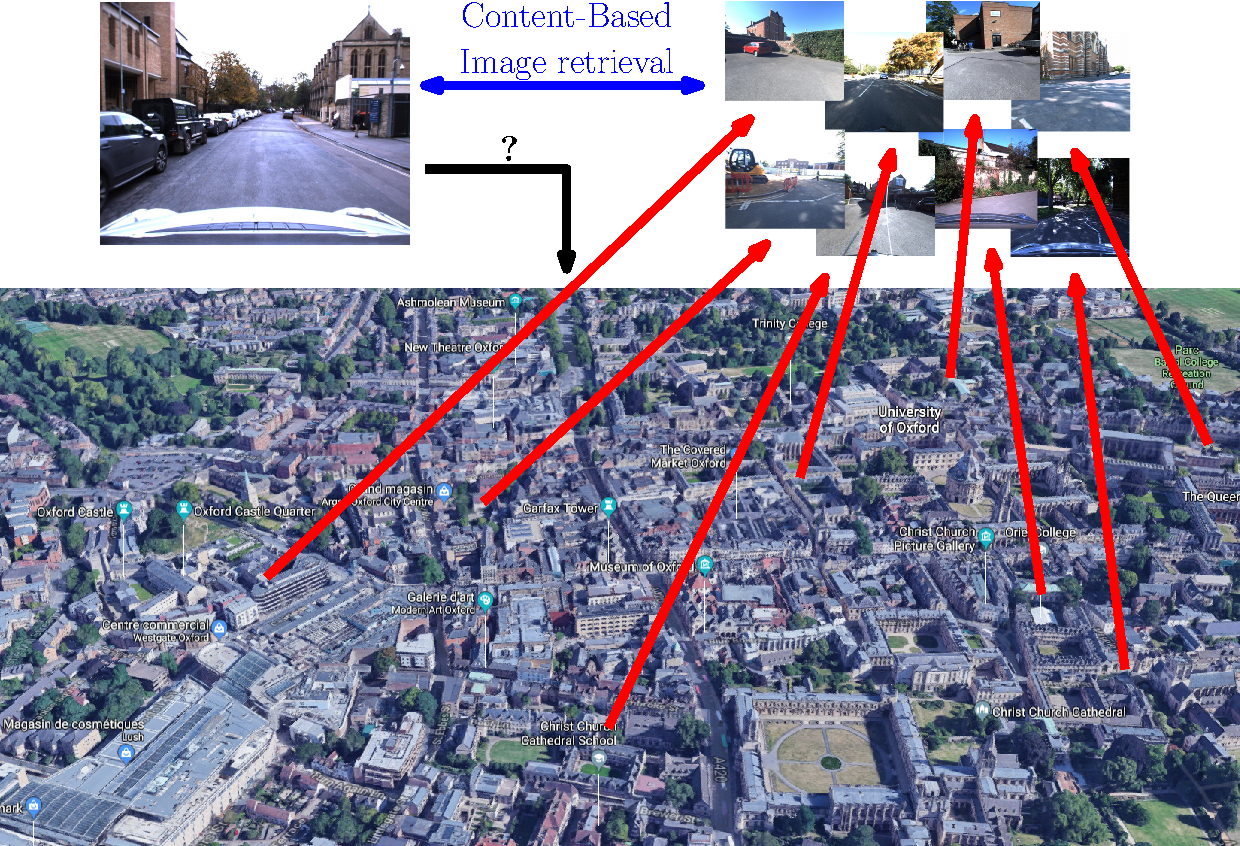
\includegraphics[width=\linewidth]{vect/intro/fig1/intro_poster}
    \end{figure}
    
     \begin{enumerate}
       \item Collect geolocalized images on the area of interest.
       \item Cast the image localization problem as an \textbf{image-retrieval problem}.
       \item Transfer the pose of the closest retrieved candidate to the query.
     \end{enumerate}
  \end{block}
  
  \vspace{2cm}

  \begin{block}{Challenge in visual based localization}
     Drastic \textbf{visual changes} occur due to season/day-night cycles.

	\begin{figure}
		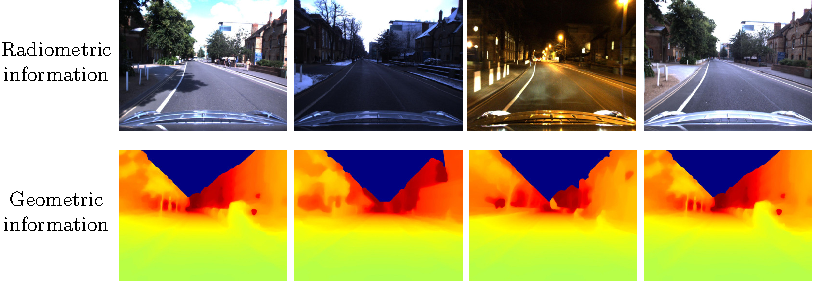
\includegraphics[width=\linewidth]{vect/intro/fig4/radvsdepth}
	\end{figure}

	However, {geometric information} still remains the same. Unfortunately, geometric information is not always available.

	\textbf{How to use partial geometric information to improve image descriptor for localization?}
  \end{block}
  
  \vspace{2cm}

  \begin{block}{System components}
    \begin{minipage}{0.75\linewidth}
        \centering
    	\begin{figure}
		  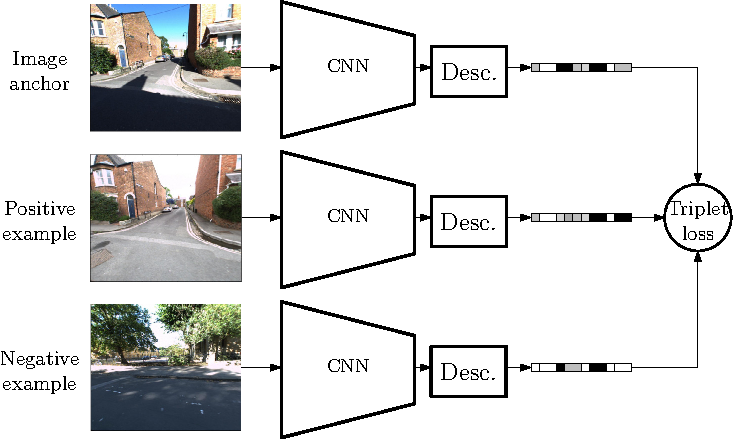
\includegraphics[width=\linewidth]{vect/method/fig2/3n}
		\end{figure}	
    \end{minipage}\hfill
    \begin{minipage}{0.23\linewidth}
      	{\footnotesize Trainable global image descriptor} 
    \end{minipage}
    
    \begin{minipage}{0.75\linewidth}
        \centering
    	\begin{figure}
		  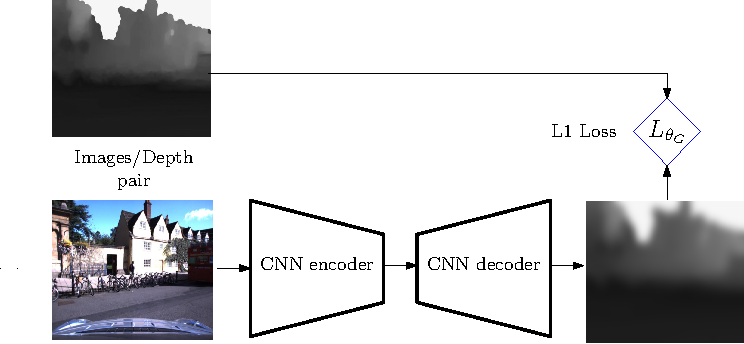
\includegraphics[width=\linewidth]{vect/method/fig3/enc_dec}
		\end{figure}	
    \end{minipage}\hfill
    \begin{minipage}{0.23\linewidth}
      	{\footnotesize Depth from monocular network}   
    \end{minipage}
    \vspace{1.5cm}
    
    \begin{minipage}[t]{0.52\linewidth}
    \textbf{Global image descriptor}
    
    {Triplet loss} penalizes difference between anchor \& positive example and similarity between anchor \& negative example:
	\begin{multline*}
     	L = \mathrm{max}\left(\lambda + \norm{f(q_{im}) - f(q_{im}^+)}_2 \right. \\	
	\left. - \norm{f(q_{im}) - f(q_{im}^-)}_2, 0 \right),
	\end{multline*}
where $\{q_{im}, q_{im}^+, q_{im}^-\}$ is an image triplet, $f(x_{im})$ the global descriptor of image $x_{im}$ and $\lambda$ an hyper-parameter controlling the margin between positive and negative examples.
    \end{minipage}\hfill
    \begin{minipage}[t]{0.45\linewidth}
	\textbf{Depth from monocular}
	
    We use an encoder/decoder architecture to generate depth map from monocular images.
    
	Training is done in a supervised manner by minimising $L_1$ loss function:
	\begin{equation*}
     	L = \norm{G(I) - D_I)}_1,
	\end{equation*}
where $G(I)$ is the generated depth map from image $I$ and  $D_I$ the ground truth depth map associated to image $I$.    
    \end{minipage}
  \end{block}
  
\end{column}

\separatorcolumn

\begin{column}{\colwidth}  

	\vspace{2cm}
	
		\begin{minipage}[t]{0.20\linewidth}
			\centering
			
\includegraphics[width=\linewidth]{images/logos/ign_logo} 
		\end{minipage}\hfill
		\begin{minipage}[t]{0.19\linewidth}
			\centering
			
\includegraphics[width=\linewidth]{images/logos/cnrs} 
		\end{minipage}\hfill
		\begin{minipage}[t]{0.32\linewidth}
			\centering		
			
\includegraphics[width=\linewidth]{images/logos/ubfc} 
		\end{minipage}\hfill
		\begin{minipage}[t]{0.20\linewidth}
			
\includegraphics[width=\linewidth]{images/logos/vibot}
		\end{minipage}\hfill
	
	\vspace{2cm}
	
  \begin{block}{Learning through missing modality}
    \begin{figure}
		\centering
		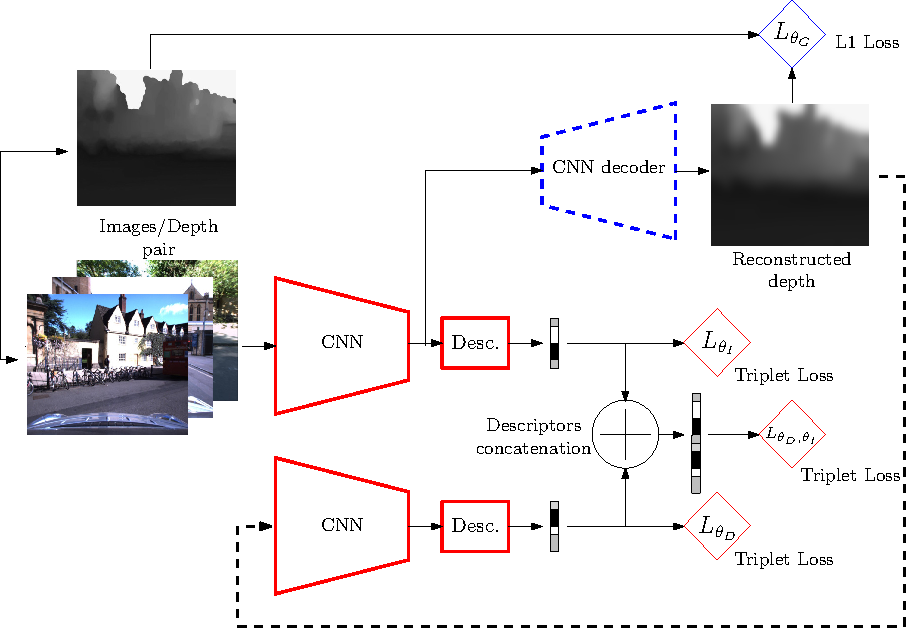
\includegraphics[width=\linewidth]{vect/method/fig3/final_color}	    
    \end{figure}
    
    \begin{enumerate}
      \item We use triplet loss to produce a strong image descriptor.
      \item Latent image representation is given to a CNN decoder to reproduce the scene geometry.
      \item We use a second CNN to produce a strong depth map descriptor.
      \item Final descriptor is obtained by concatenating image and depth map descriptors.
    \end{enumerate}        
    
    Our proposal is trained with two different types of data:
    \begin{itemize}
    	\item \textcolor{red}{Image triplet}
    	\item \textcolor{blue}{Pair of image and associated depth map}
    \end{itemize}
  \end{block}

  \vspace{1.5cm}
  
  \begin{block}{System deployment}
	\begin{figure}
	  \centering
	  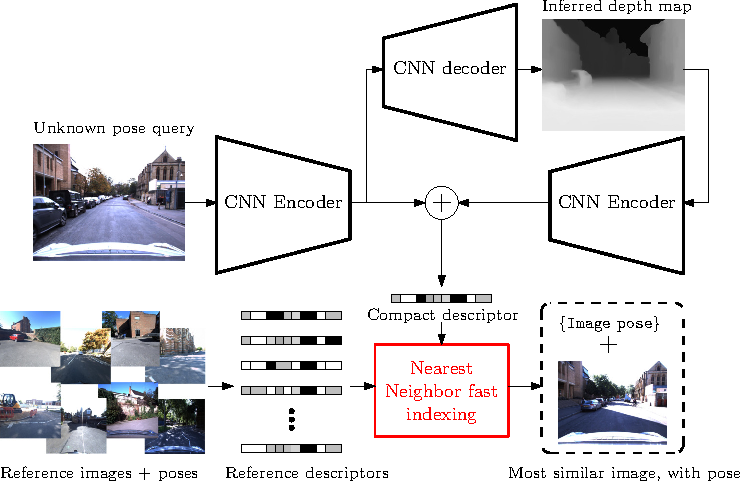
\includegraphics[width=\linewidth]{vect/method/fig4/final}
	\end{figure}

	\textbf{The depth information is only needed during the training step!}
  \end{block}
	
  \vspace{1.5cm}
  	
  \begin{block}{Dataset \& Implementation}
  
  Training parameters:
  \begin{itemize}
  	\item \texttt{pytorch} framework
  	\item adam optimizer with lr=0.0001 and wd=0.001
  	\item batches of 10 or 25 triplets, trained up to 50 epochs
  \end{itemize}
  
	\begin{table}
  \begin{tabular}{l | l || l | l}
  	\multicolumn{2}{c}{\textbf{Encoder}} & \multicolumn{2}{c}{\textbf{Descriptor}} \\
  	\hline
	Alexnet (A) & Resnet18 (Rt) & MAC~\cite{Radenovic2017} & NetVLAD~\cite{Arandjelovic2017} \\
  \end{tabular}
  \caption{Four possible combination of encoder/descriptor}
  \end{table}
  
  Competitors:
  \begin{itemize}
  	\item Only RGB (dotted line)
  	\item Hallucination network~\cite{Hoffman2016} (plain line with cross)
  \end{itemize}
  
	We train and test our proposal on RobotCar dataset with 4 different localization scenarios~\cite{Maddern2016}.
	\begin{figure}
		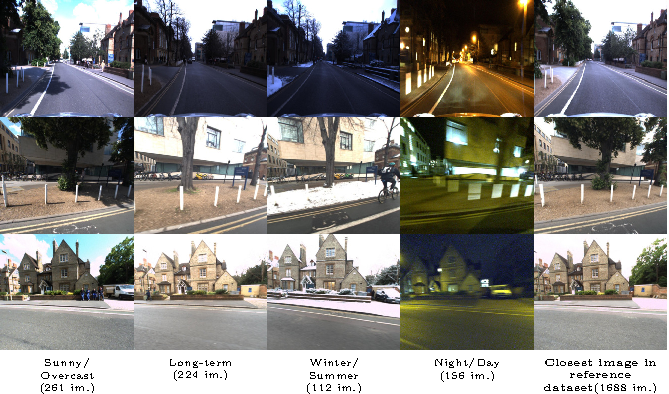
\includegraphics[width=\linewidth]{vect/res/dataset}
	\end{figure}
  \end{block}
\end{column}

\separatorcolumn

\begin{column}{\colwidth}
  \begin{block}{Results}
  		\begin{minipage}{0.49\linewidth}
	  		\centering
	  		Sunny
	  		
			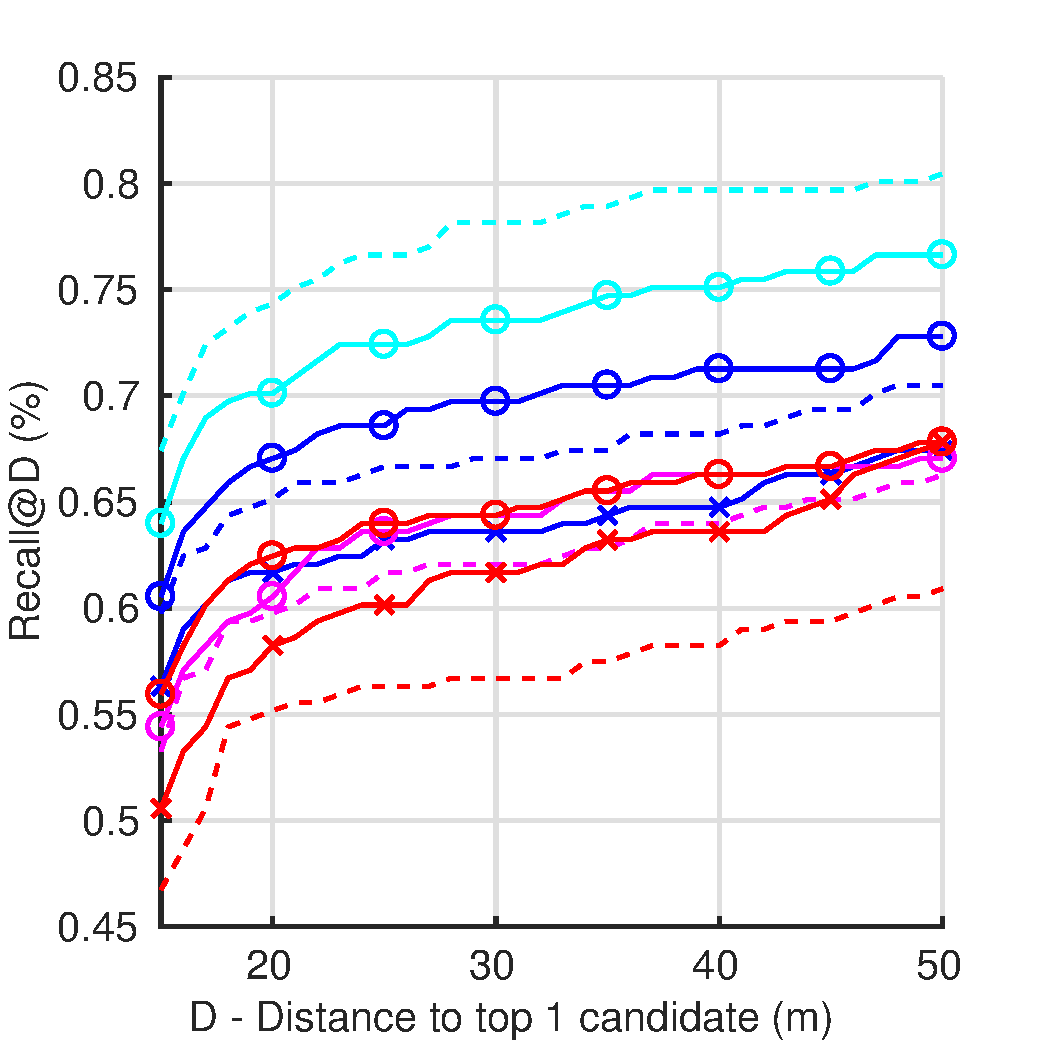
\includegraphics[width=\linewidth]{vect/res/sunny}
		\end{minipage}\hfill
		\begin{minipage}{0.49\linewidth}
	  		\centering
			Long-term
			
			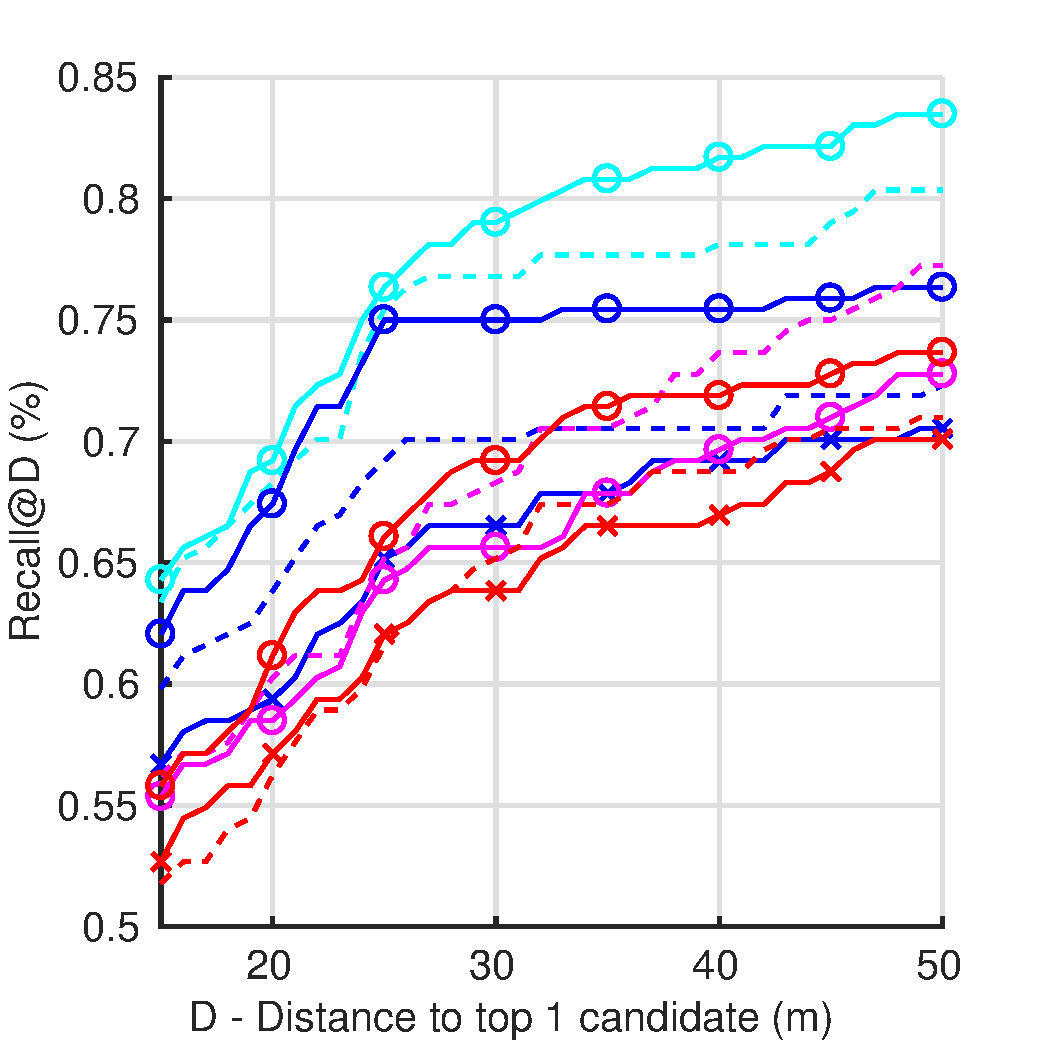
\includegraphics[width=\linewidth]{vect/res/lt}
		\end{minipage}
		
		\begin{minipage}{0.49\linewidth}
	  		\centering
			Snow
			
			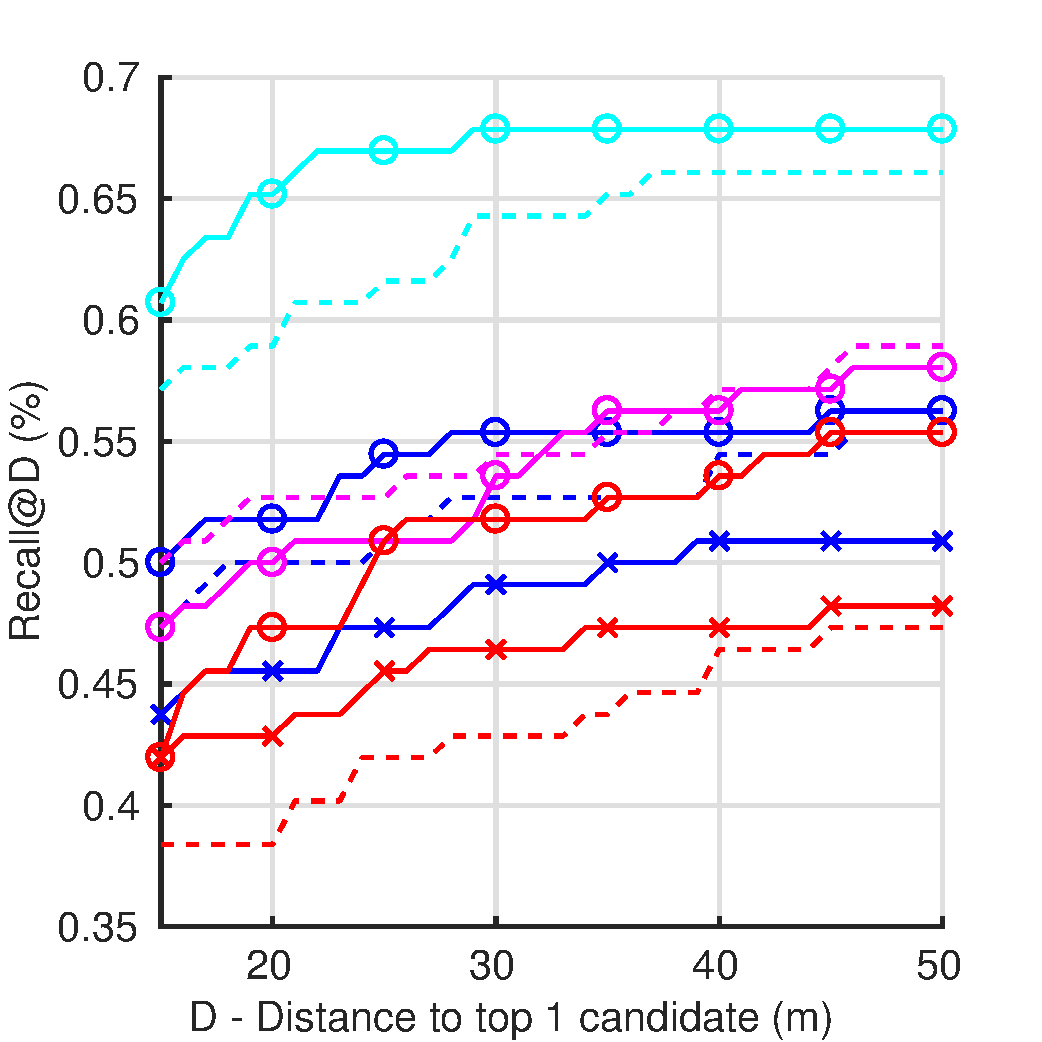
\includegraphics[width=\linewidth]{vect/res/snow}
		\end{minipage}\hfill
		\begin{minipage}{0.49\linewidth}
	  		\centering
	  		Night
	  					
			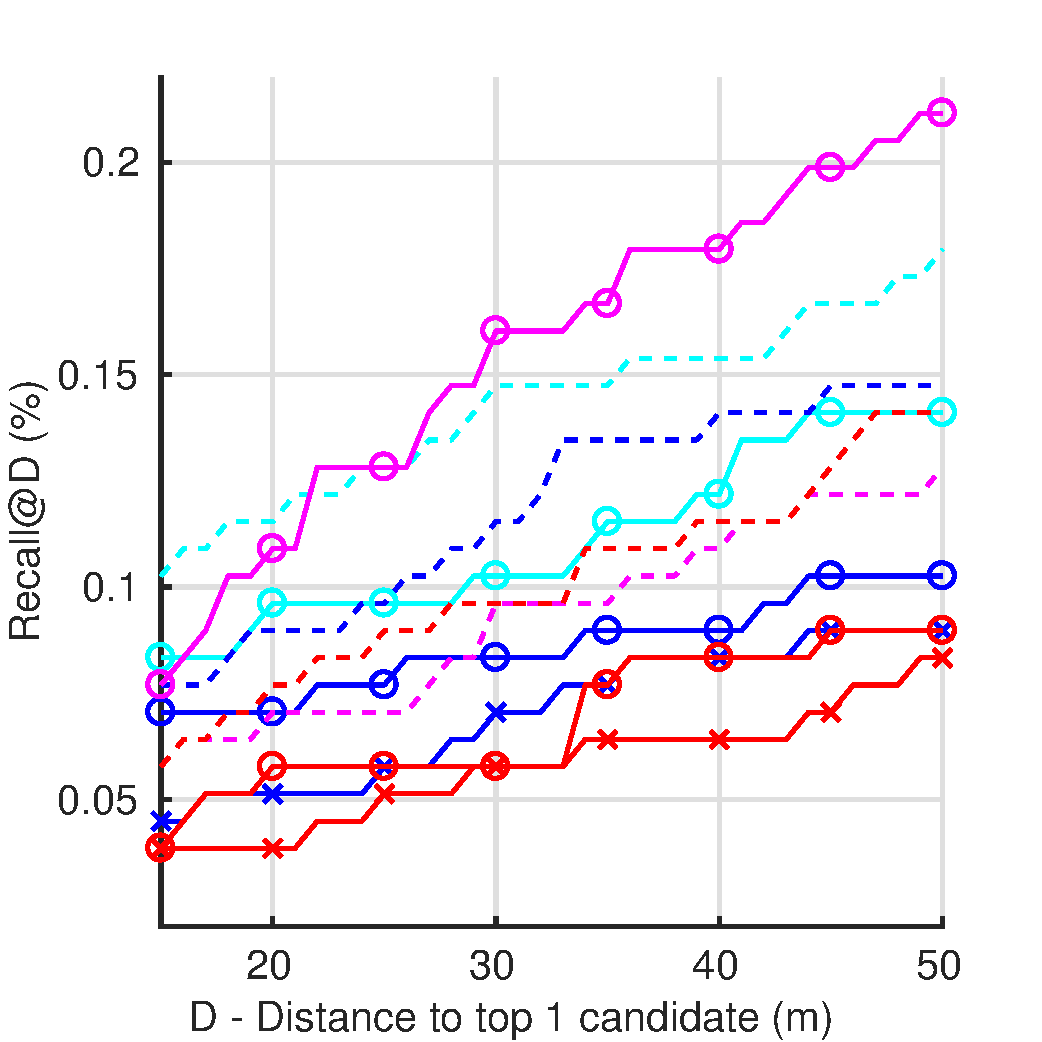
\includegraphics[width=\linewidth]{vect/res/night}
		\end{minipage}
		
		\begin{minipage}{0.49\linewidth}
     		\centering
			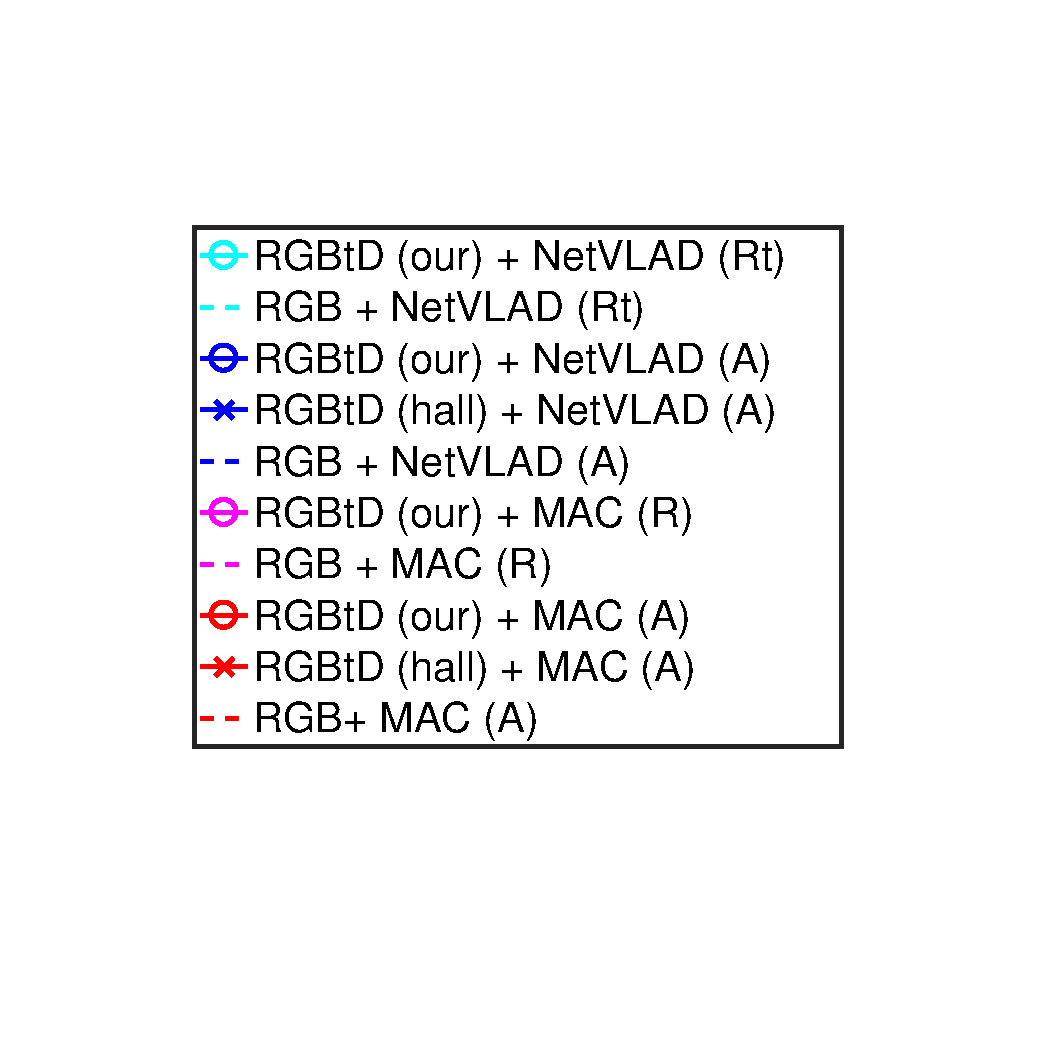
\includegraphics[trim={90 140 95 100},clip,width=0.7\linewidth]{vect/res/legend}	\hfill
		\end{minipage}\hfill
		\begin{minipage}{0.49\linewidth}
			\textbf{Metric:} we compute the distance between \textbf{the top ranked} returned database image position and the query ground truth position and report the percentage of queries well located under a threshold D.
		\end{minipage}
  \end{block}
  
  \begin{block}{Improving night to day localization}
     Our network is \textit{not able} to generate proper depth maps from night images.
  \begin{figure}
	\centering
    	\begin{minipage}{0.15\linewidth}
			\raggedright \footnotesize
			Input
		\end{minipage}
		\begin{minipage}{0.7\linewidth}
			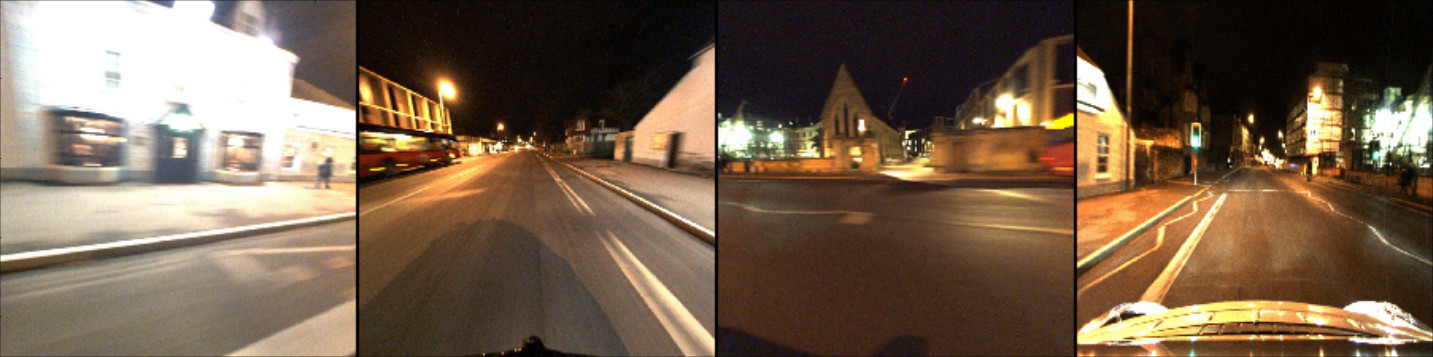
\includegraphics[width=\linewidth]{im/res/night_input}
		\end{minipage}
		
    	\vspace{-0.5cm}
		\begin{minipage}{0.15\linewidth}
			\raggedright \footnotesize
			GT
		\end{minipage}
		\begin{minipage}{0.7\linewidth}
			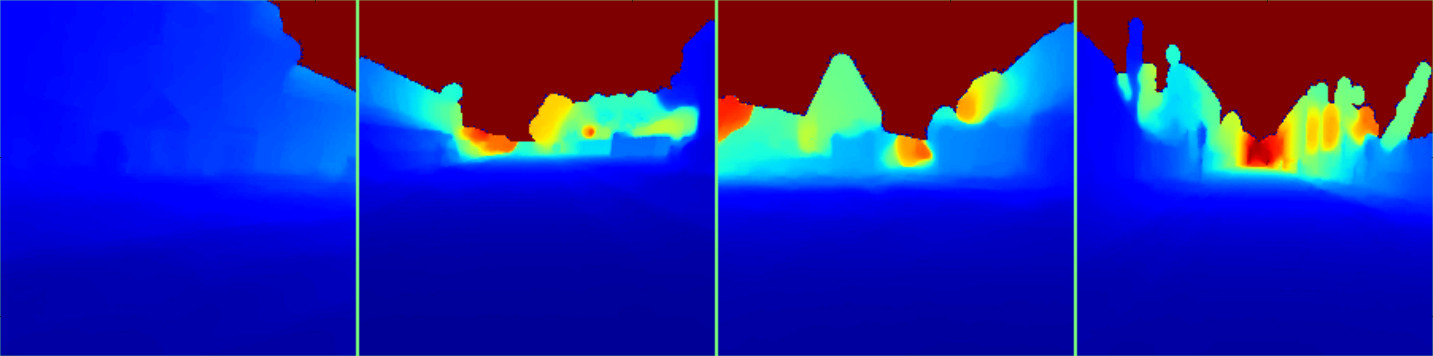
\includegraphics[width=\linewidth]{im/res/night_gt}
		\end{minipage}
		
    	\vspace{-0.5cm}
		\begin{minipage}{0.15\linewidth}
			\raggedright \footnotesize
			Out
		\end{minipage}
		\begin{minipage}{0.7\linewidth}
			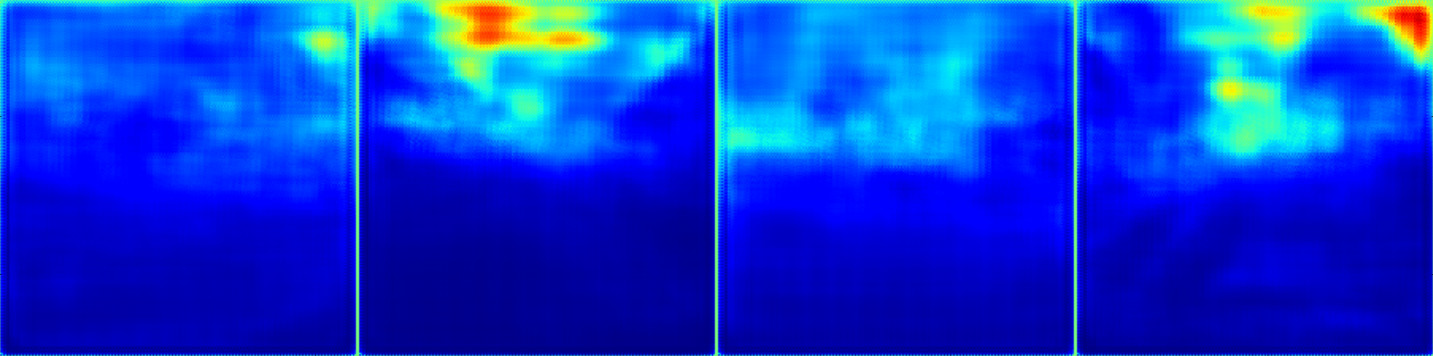
\includegraphics[width=\linewidth]{im/res/night_noft}
		\end{minipage}

		\vspace{-0.5cm}
		\begin{minipage}{0.15\linewidth}
			\raggedright \footnotesize
   			Out + ft
		\end{minipage}
		\begin{minipage}{0.7\linewidth}
			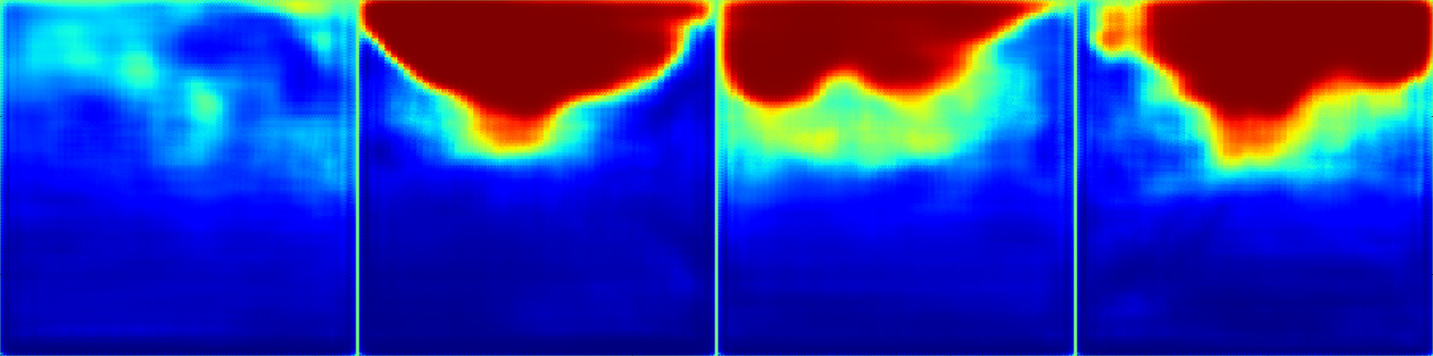
\includegraphics[width=\linewidth]{im/res/night_ft}
		\end{minipage}
    \end{figure}
    
	 Thanks to the design of our method, we can improve generation performances of the decoder without impacting the descriptors networks.
  
      \begin{minipage}{0.49\linewidth}
	  		\centering
	  		Night
	  		
			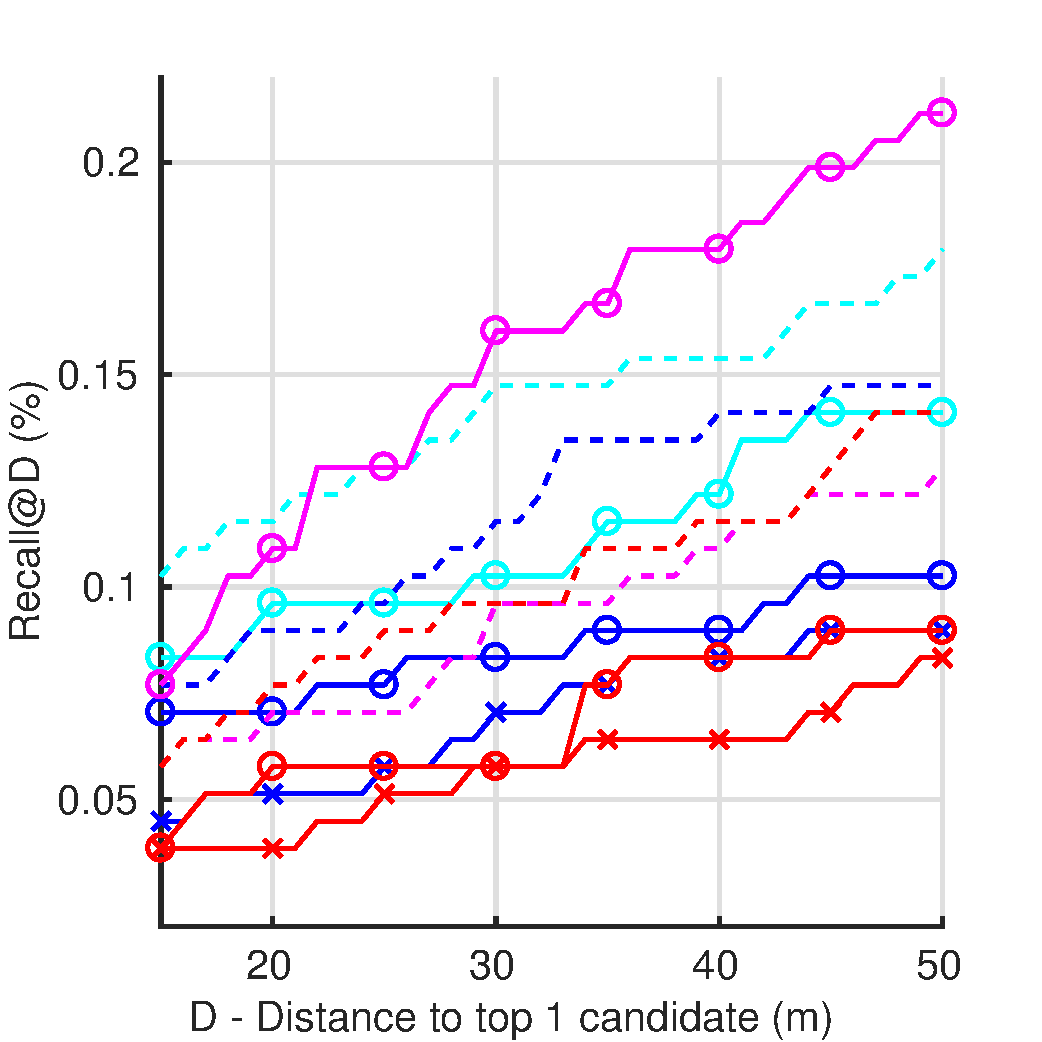
\includegraphics[width=\linewidth]{vect/res/night}
		\end{minipage}\hfill
		\begin{minipage}{0.49\linewidth}
	  		\centering
			Night (after ft)
			
			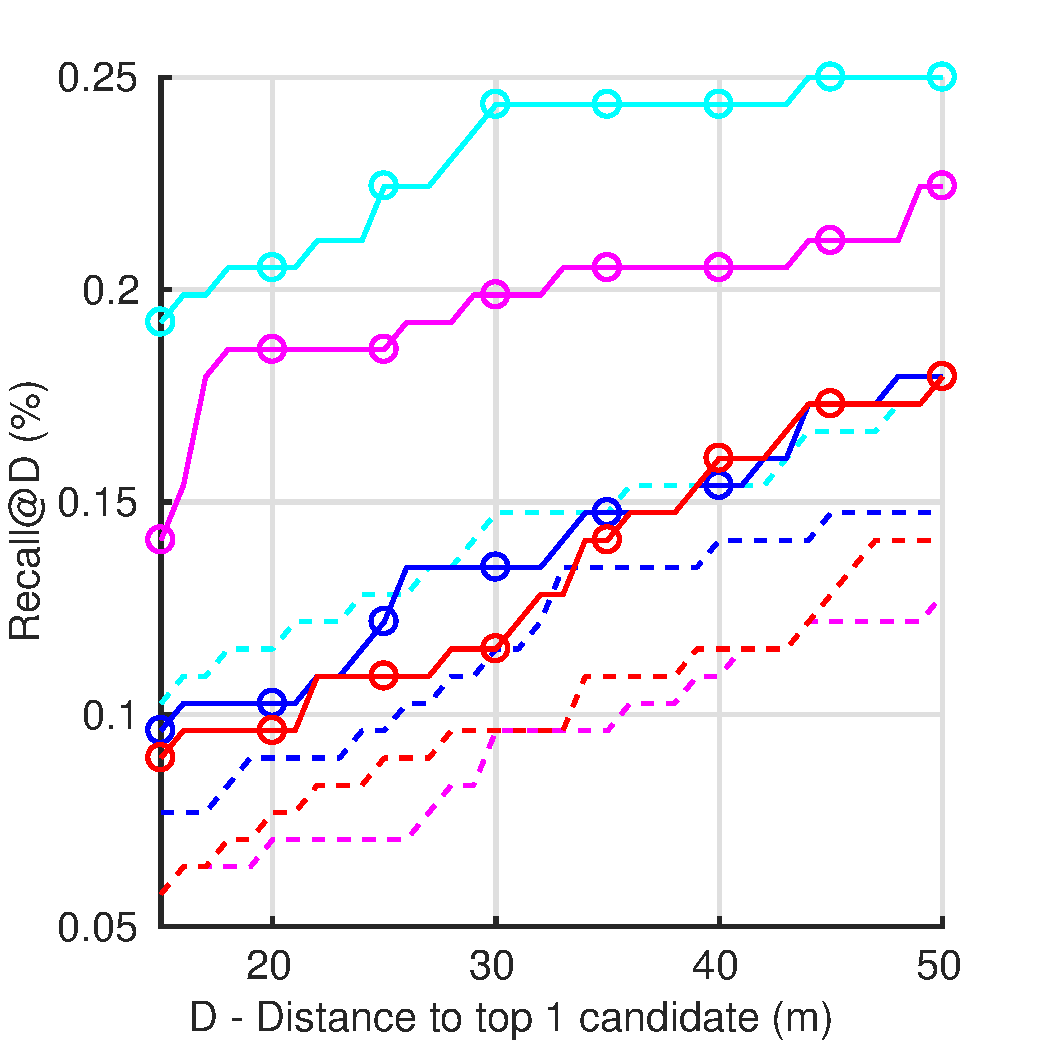
\includegraphics[width=\linewidth]{vect/res/nightft}
		\end{minipage}		
  \end{block}

  \begin{alertblock}{Perspectives}
	\begin{itemize}
		\item Test our proposal on other modalities.
		\item Investigate a less trivial descriptors fusion method.
		\item Implement our method for other visual localisation tasks (e.g. direct pose regression).
	\end{itemize}
  \end{alertblock}  

  \begin{block}{Acknowledgments}
	We would like to acknowledge the French ANR project pLaTINUM (ANR-15-CE23-0010) for its financial support. We also gratefully acknowledge the support of NVIDIA Corporation with the donation of the Titan Xp GPU used for this research.
  \end{block}
  
  \begin{block}{References}
    \footnotesize{\bibliographystyle{plain}\bibliography{../slides/bib/mendeley.bib}}
  \end{block}
\end{column}

\separatorcolumn
\end{columns}
\end{frame}

\end{document}
